This chapter will dissect the LHC machine which accelerates particles at a speed close to the speed of light before they collide with each other. The aim of Run II of LHC was to study all Higgs production modes, decay modes and accuracy in studying its properties. Also if there are deviations in the data accumulated from the one predicted in Standard Model which will mark new physics such as supersymmetry, dark matter and dark energy, antimatter deficit compared to matter and how quark-gluon plasma are the source behind particles that make the matter of Universe. We have used Monte Carlo (MC) samples produced from Run II from 2016 till 2018 in our thesis for data analysis.\\
\section{Large Hadron Collider}
Large Hadron Collider (LHC) is the world's biggest and most dynamic machine ever built. It is absurd, as the world's largest machine was built to comprehend the smallest particle known to mankind. It runs approximately $\sim$100m underground and travels 27 km in circumference which consists of superconducting magnets and accelerating compartments, shown in Fig.\ref{fig:lhc}, which give the particles an energy boost along the path. It accelerates two beams of protons, circulating the ring, in opposite directions induced with ultrahigh vacuum. These protons are circulated by the strong magnetic field used for ‘bending’ and a series of other magnets that are used for controlling and focusing the beams. The superconducting magnets are made from electric cables which reduce energy loss and resistance in superconducting state. When the particles are just about to collide a magnet is used to ``squeeze'' the particles in the beam's cross section to increase the collision rate known as integrated luminosity.\\
\begin{figure}
    \centering
    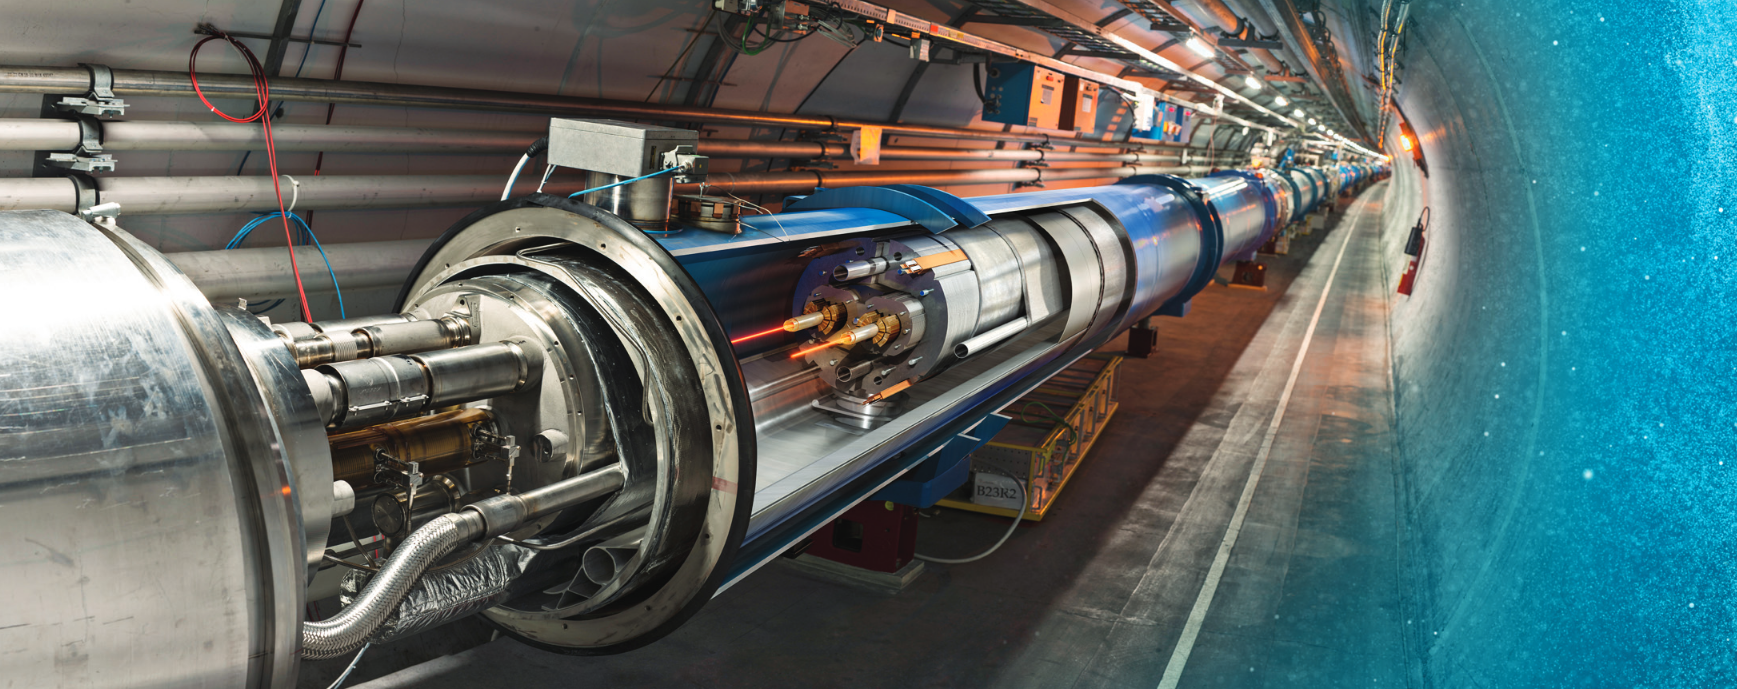
\includegraphics[scale=0.26]{images/lhci.png}
    \caption{LHC at CERN, Geneva}
    \label{fig:lhc}
\end{figure}
Protons are accelerated up to the necessary energies, through a series of smaller accelerators shown in Fig.\ref{fig:accom}. The process starts with the 50 MeV LINAC2 which shoots the protons into a multi-ring booster synchrotron that accelerates them up to 1.4 GeV. After which the protons are directed to the Proton Synchrotron (PS) machine accelerating the particles up to 26 GeV and generate the bunching and spacing that the LHC requires. To accelerate the beam from 26 GeV up to 450 GeV the beam is then injected into the Super Proton Synchrotron (SPS). In the SPS the protons are fed into one of the LHC rings. Before the LHC accelerates these protons up to their final energies, this process is repeated 24 times, 12 times to fill each of the two rings. Once the LHC has accelerated these proton bunches to their final energies, the beams are gradually brought together so that they will collide inside the four experiments. \\
\begin{figure}[h]
\centering
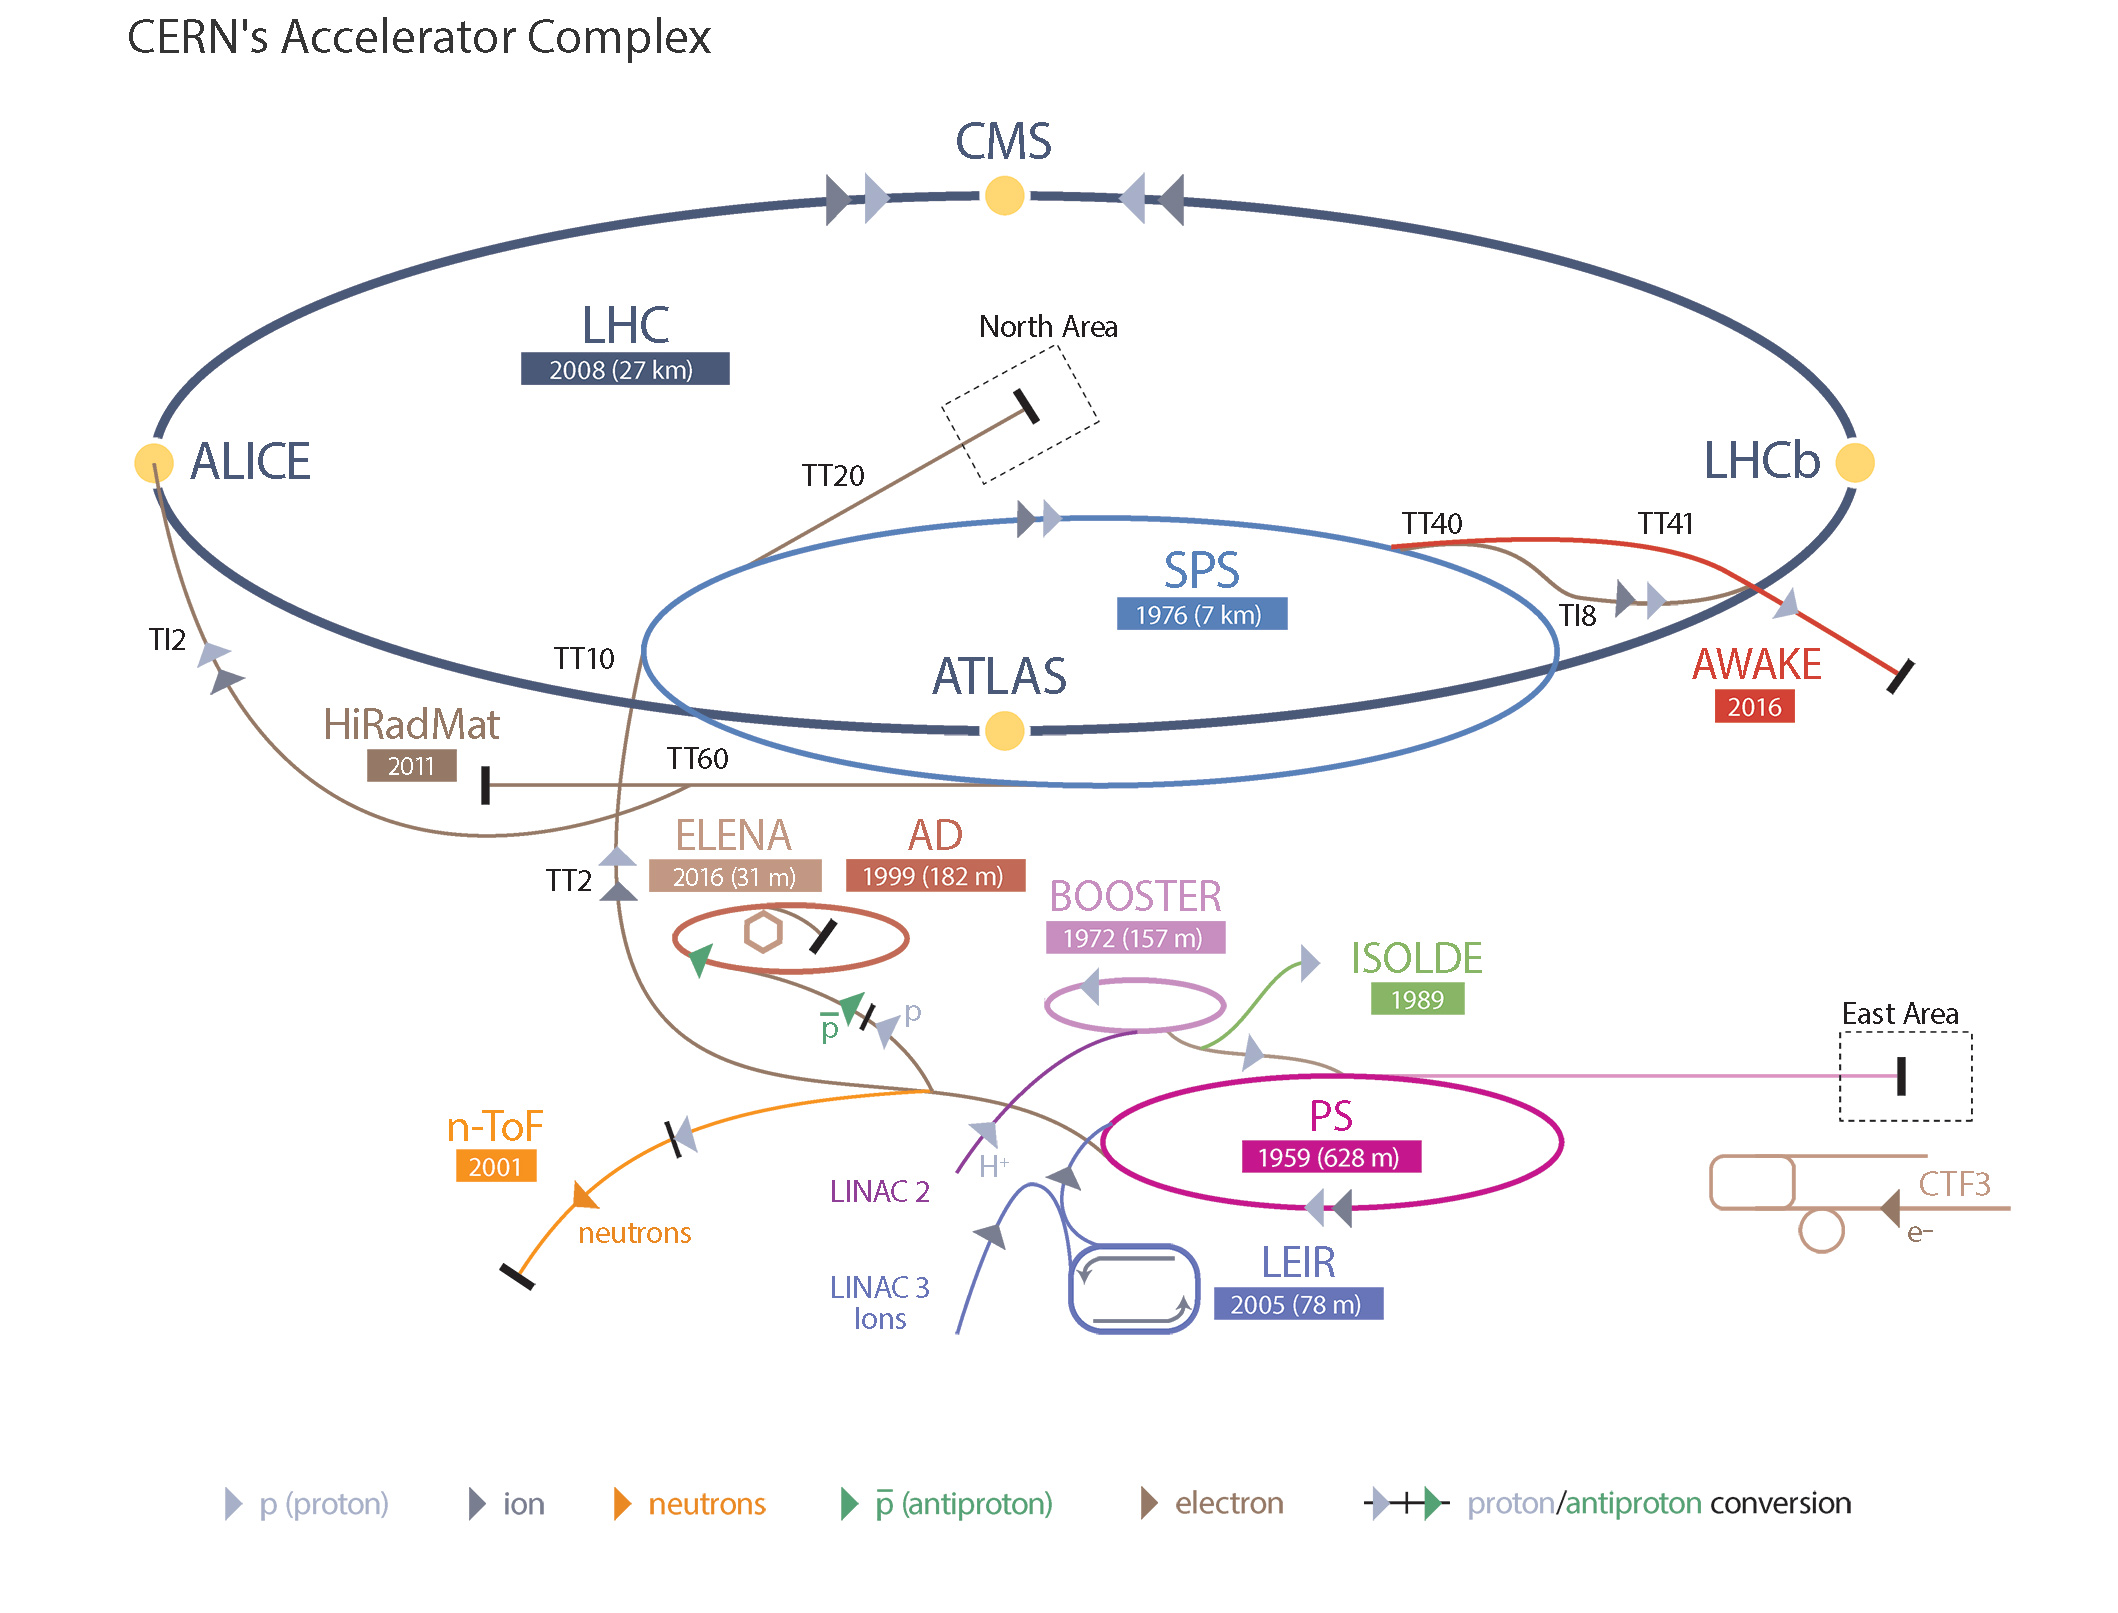
\includegraphics[scale=0.1]{images/acc.jpg}
\caption{This CERN accelerator complex. Experiments at LHC: ALICE, ATLAS, CMS, LHCb \cite{<acc>}.}
\label{fig:accom}
\end{figure}
Theses detectors observe and categorize the particles that are produced when these protons (ions) are collided with each other. Currently, the four experiments at the LHC are: The Compact Muon Solenoid (CMS), A Toroidal LHC Apparatus (ATLAS), Large Hadron Collider beauty (LHCb) and Large Ion Collider Experiment (ALICE). The ATLAS and CMS detectors are high luminosity, all-purpose detectors constructed to test many different aspects of the SM, including the Higgs boson. LHCb looks specifically at bottom (beauty) quark interactions and while ALICE is designed for ion collisions.
\section{CMS Detector}
Compact Muon Solenoid as shown in Fig.\ref{fig:dec} is a multipurpose detector where its key characteristics are defined in its name:
\begin{itemize}
    \item \textbf{Compact}: it has small dimensions compared to its mass, a compact detector as the tracker and calorimeter are within superconducting coil.
    \item \textbf{Muon}: it has advanced muon detection system, it is developed with muons triggers and muon chambers which detect muon signatures for events such as; Higgs decays to four muons.
    \item \textbf{Solenoid}: solenoidal superconducting magnet, the largest solenoid magnet (B = 4T) in the world which is producing a field 100,000 times the Earth's magnetic field.
\end{itemize}
\begin{figure}[h]
\centering
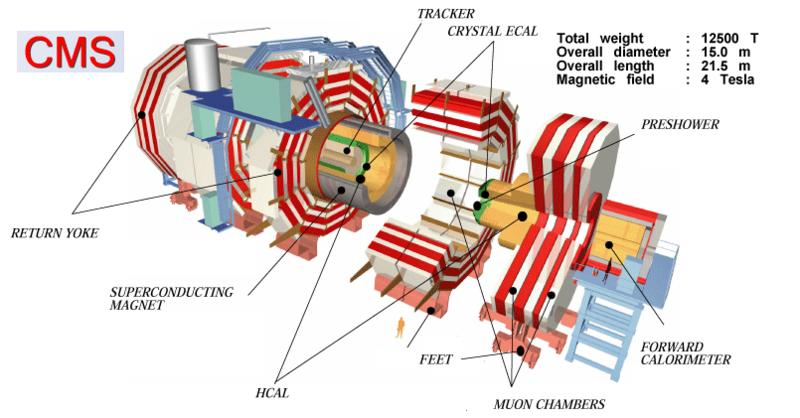
\includegraphics[scale=0.4]{images/9803027.jpg}
\caption{The CMS Detector \cite{<cms>}}
\label{fig:dec}
\end{figure}
\subsection{Tracker}
Tracker is the central hollow vacuum path of the LHC, with silicon sensors that are finely segmented. These silicon pixels and silicon strips, track charged particles and measure their momenta. They can also give the positions of decay of long-lived unstable particles. The CMS silicon tracker consists of two tracking devices which utilize semiconductor technology: the inner pixel and the outer strip detectors.\\
The tracker detector is in the middle of CMS, where the beams collide in the range of 4cm to 110cm in radius and $\sim$280cm along the beam axis. The CMS tracker is built to reproduce objects such as high $p_{T}$ hadrons, muons and electrons along high precision and an apt resolution of momentum. Decay vertices of long-lived unstable particles can also be measured. This is the reason behind the use of all-silicon for the tracking system. Charge particles are tracked and their momentum is efficiently measured by the finely segmented silicon sensors. The CMS tracking system is illustrated in Fig.\ref{fig:CMS Tracking System}.
\begin{figure}[h]
     \centering
     \begin{subfigure}[b]{0.45\textwidth}
         \centering
         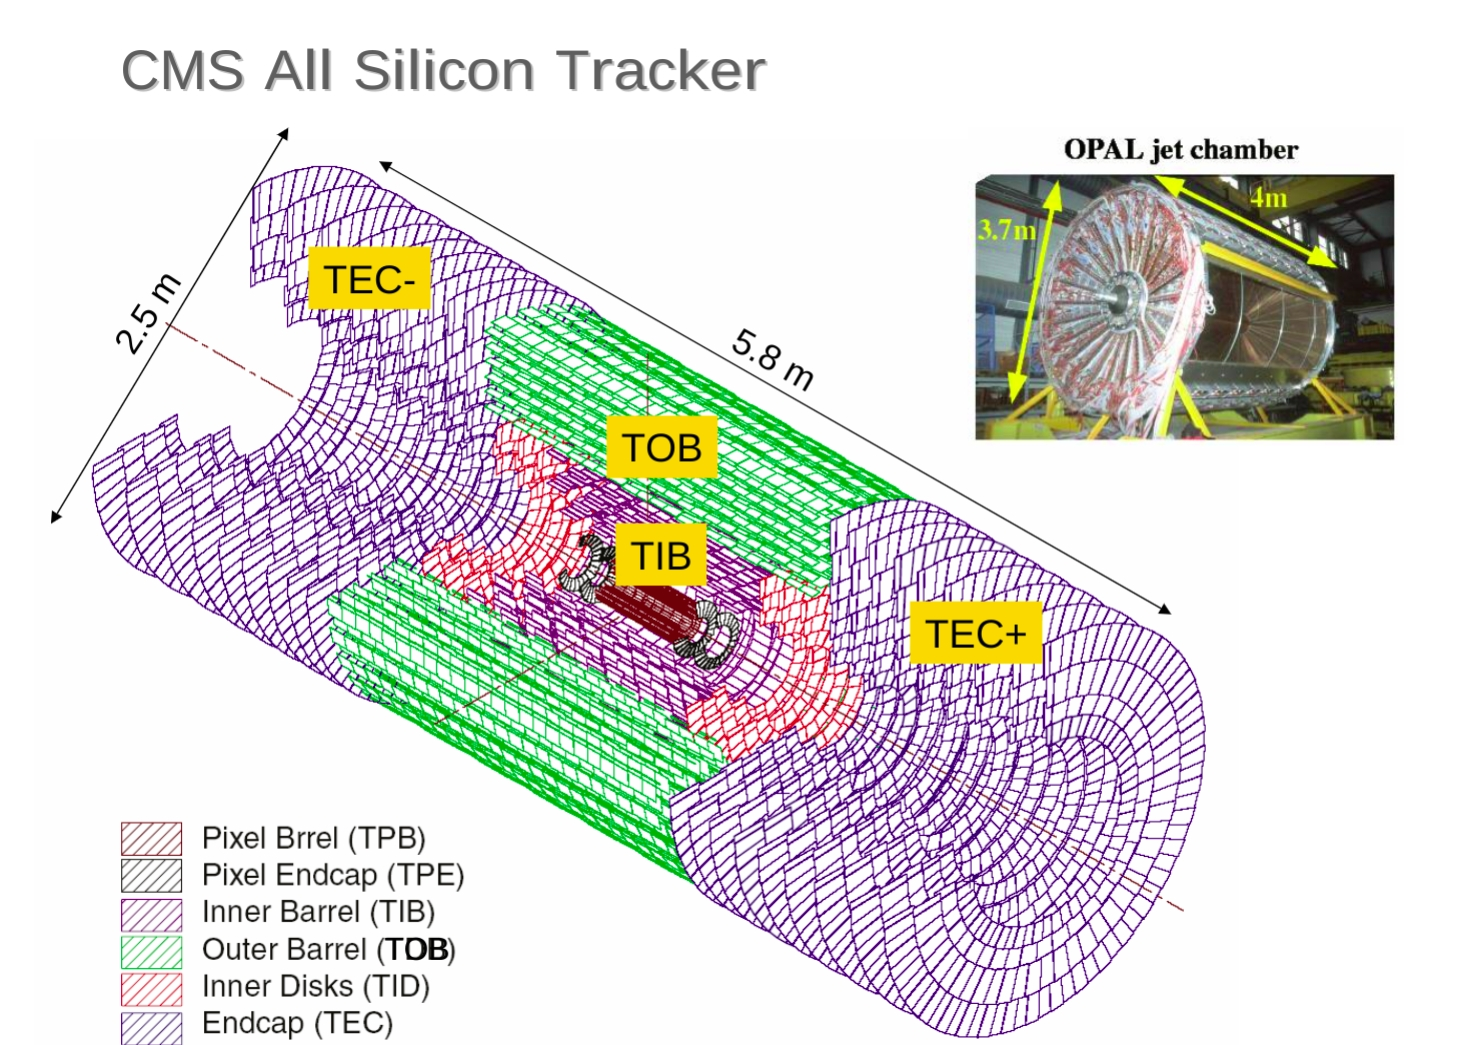
\includegraphics[width=\textwidth]{images/Track1.jpg}
         \caption{The Tracking System}
         \label{fig:track1}
     \end{subfigure}
     \hfill
    \begin{subfigure}[b]{0.45\textwidth}
         \centering
         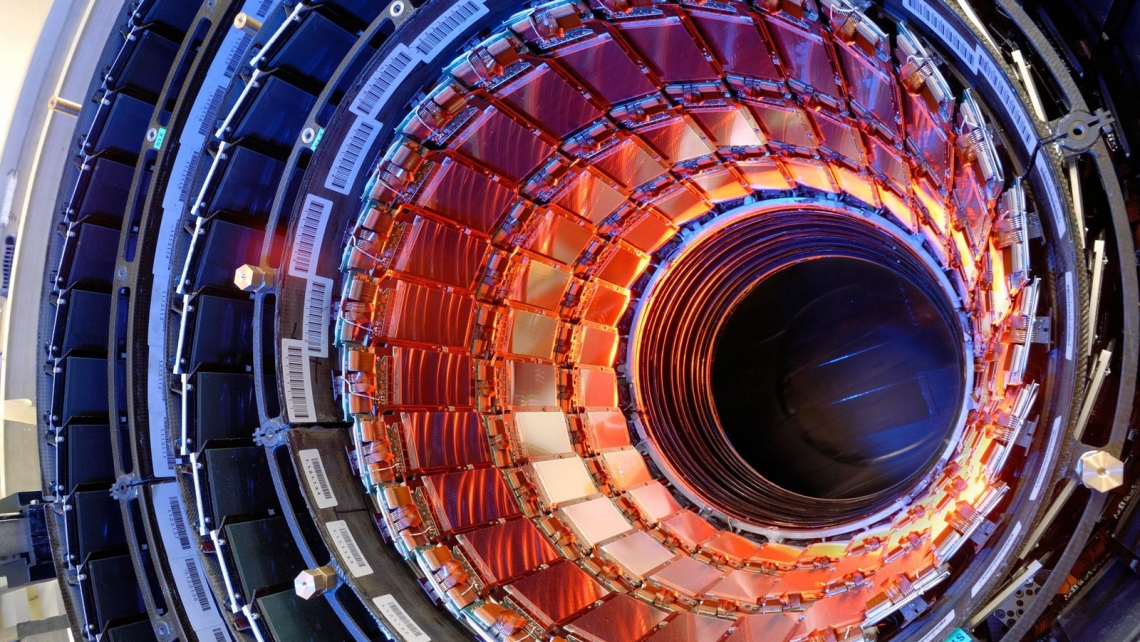
\includegraphics[width=\textwidth]{images/Track2.jpg}
         \caption{CMS Tracker}
         \label{fig:track2}
     \end{subfigure}
     \hfill
     \caption{Visualising CMS Tracker}
        \label{fig:CMS Tracking System}
\end{figure}
The tracker covers the region with pseudorapdity (the particle's angle relative to the beam axis) $|\eta|< 2.5$. High $p_{T}$ resolution tracks are reproduced  $\delta P_{T}$ /$P_{T}$ = (15$P_{T}$/TeVc + 0.5) in the core area $|\eta| < 1.6$, with resolution $\delta P_{T}$ /$P_{T}$ = (60$P_{T}$ /TeVc + 0.5) when $|\eta|\sim$ 2.5.
The inner pixel device contains $4.4 \times 10^{6}$ pixels as a square with each side 150 µm in length. The resolution of dimensions is 15 µm. The outer strip device includes strips amounting to $25 \times 10^{3}$. The barrel has ten strip layers and three pixel layers. Where as the endcaps have nine outer forward silicon detectors (TOB), three inner discs (TID) and two pixel layers.
\subsection{Electromagnetic Calorimeter}
The (ECAL) electromagnetic calorimeter has been equipped to accurately detect positions and energies for photons and electrons. It also measures the energies from the showers of hadrons and jets which deposit portion of their energies in ECAL. The ECAL is a homogeneous calorimeter and its crystals are made up of lead tungstate (PbWO4). It has small radiation distance ($X_0 = 0.89 \times 10^{-2}$) and an enormous density ($8.2 g/cm^3$), and small Moli`ere radius ($R_{M} = 2.19 \times 10^{-2}$). Endcap (EE) and barrel (EB)  are the two regions of the ECAL. The EB encompasses the domain $|\eta| < 1.48$ and has 61,000 crystals. There are 36 superunits in the EB, and every unit consists of four modules illustrated in Fig.\ref{fig:e1}. Every crystal of lead tungstate consists of front facing area of 22 × 22 $mm^2$ and 26 × 26 $mm^2$ back area and all of them are 23 cm long, about 26$X_0$. Lead tungstate crystals are tilted along the beam axis at $3^{\circ}$. Avalanche photo diodes (APD) comprehend signals computed behind the crystals in the EB. The EE covers area between $1.5 < |\eta| < 3.0$. \\
\begin{figure}[h]
     \centering
     \begin{subfigure}[b]{0.55\textwidth}
         \centering
         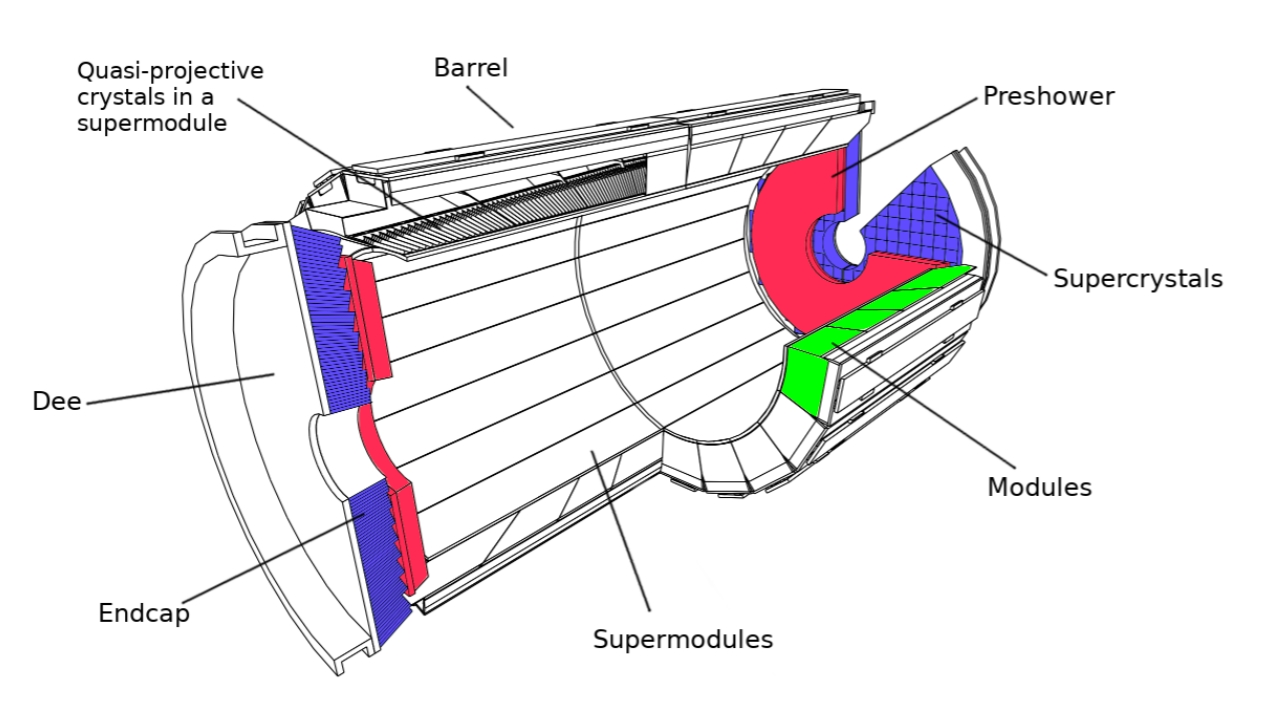
\includegraphics[width=\textwidth]{images/ecal1.jpg}
         \caption{ECAL Geometry}
         \label{fig:e1}
     \end{subfigure}
     \hfill
    \begin{subfigure}[b]{0.4\textwidth}
         \centering
         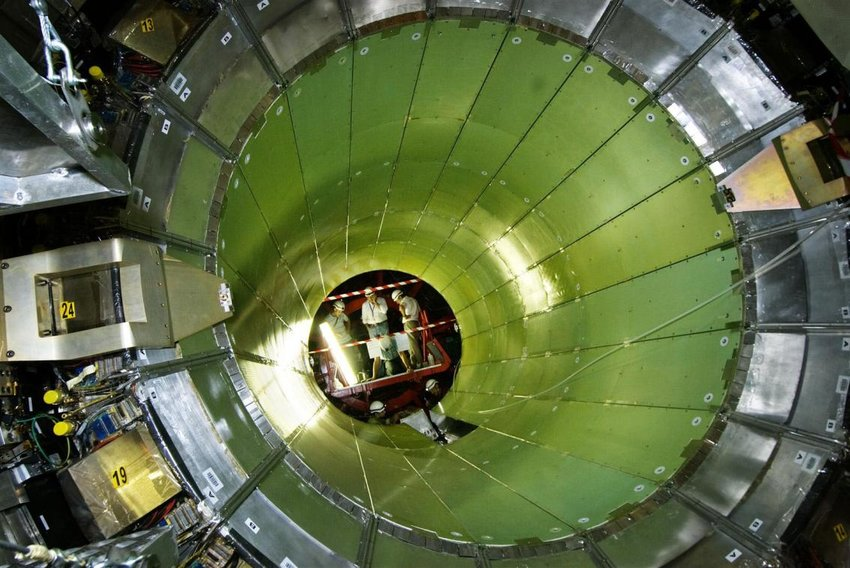
\includegraphics[width=\textwidth]{images/ecal2.png}
         \caption{Insertion of the last CMS ECAL supermodules in the ECAL Barrel}
         \label{fig:e2}
     \end{subfigure}
     \hfill
     \caption{Electronic Calorimeter}
        \label{fig:ECAL}
\end{figure}
EE has 73000 crystals and vacuum photo triodes (VPT) are used for reading the signals at crystal's back in the EE. At the face of EE, a preshower detector (ES) covers the area between $1.6 < |\eta| < 2.6$. The construction helps in dismissing $\Ppizero$ which decays into two photons. The ES minimizes this particular background in the channel where Higgs boson decays to a photon pair \cite{<ecal>}.
\subsection{Hadronic Calorimeter}
The hadronic calorimeter (HCAL), along ECAL, is also used to identify jets, hardrons and give their energy measurements. It is made up of 36 wedges, each of which weighs as much as 6 African elephants. The HCAL consists of four sub-sections: hardron barrel (HB), hadron endcap (HE), hadron outer (HO) and hadron forward (HF). In between the superconducting solenoid and ECAL the HB and HE are placed. Brass and plastic scintillating plates are the interchanging layers of which both HB and HE are made from. The HB takes over area defined by $|\eta| < 1.4$, while the HE covers area between $1.5 < |\eta| < 3.0$. Every HB tower projects a region of $\triangle\eta \times \triangle\phi$ = 0.087 × 0.087. Scintillating plates are inserted with wavelength-shifting (WLS) fibers. Light accumulated from these are detected by Hybrid Photo Diodes (HPD). Also, HB interaction length is 5.8($\lambda_I$ ) at $\eta$ = 0.\\
\begin{figure}[h]
\centering
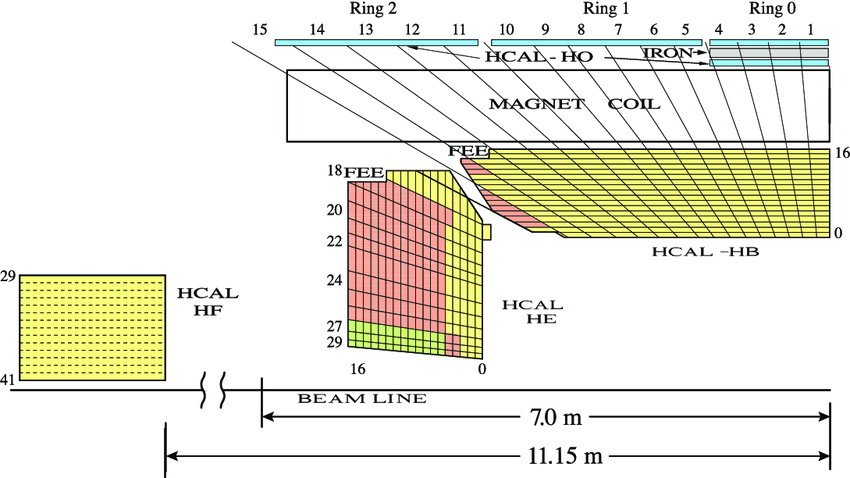
\includegraphics[scale=0.4]{images/hcal.png}
\caption{Hadron Calorimeter}
\label{fig:hcal}
\end{figure}
The tails of hadronic showers can be detected by the HO which HB cannot collect. Located in the middle of the magnet and muon system, the HO is a flash detector. It encompasses the area $|\eta| <1.26$.
At the end of HCAL, HF is located at $3.0 < |\eta| < 5.0$, which is outside the solenoid. It is built from quartz fibers which is the active medium and steel which is the absorber. Quartz fibers can tolerate the harshness of radiation, as forward calorimeters have to face particle flux of unmatched strength by the use of short fibres (1.43m) and long fibres (1.65m). The short fibers are at the front of CMS and are 22cm deep. They are placed here to detect showers created by photons and electrons. Hadrons produce signals in both segments of HCAL, leaving large traces of their energy in the 22cm depth of short fibers. HF calorimeters are built to check jets coming with high energy to an accuracy of 20\% to 30\% at 1 TeV \cite{<hcal>}.
\subsection{Superconducting Solenoid}
The experiment is built around CMS magnet. The superconducting magnets bend the trajectories of charged particles along the radius of CMS arising from the interaction point. The complication of this can be visualised by imagining the firing of two needles having 10km distance between them and even then, the interaction is as accurate as them meeting halfway but not combusting in one another. The momentum resolution of the particles can also be estimated, since the particles with high energies have less bent paths by the magnetic field. The energy loss due to magnet is reduced by cooling them to a temperature of -271.3$^{\circ}$C by liquid helium.\\
The superconducting solenoid is made of 1232 dipole magnets 23m long for bending of the beam, quadruple magnets which are 392 in amount and 5-7m in length are used for focusing the beam. The liquid helium around the solenoid, allows 19.14 kA current to flow through with negligible resistance. The flux comes back along an iron yoke containing five wheels and two end caps, each carrying three disks. The yoke mainly makes the field more homogeneous in the tracker and reduces the straying of the field by giving back the solenoid its magnetic flux. For precise reproduction and Monte Carlo (MC) event simulation, cosmic muons are used for a detail map of CMS magnetic field. The accuracy of the tracker magnetic field that has been mapped is more than 0.1$\%$.
\subsection{Muon System}
Muons are mostly seen as the end products of numerous interactions occurring at the LHC experiment. Muons travel along the whole CMS, scarcely any ionization is left along the path making it easier for muons to be identified. Recognizing muons properly and reproducing their momenta precisely, were the main construction factors in the experimental setup. The muon detecting system entails three section branching, with iron return yoke plates that allow only neutrinos and muons to transverse through: Cathode Strip Chambers (CSC) inside endcap area, Drift Tubes (DT) inside barrel area, and Resistive Plate Chambers (RPC) inside the endcap and barrel area as shown in Fig.\ref{fig:tms}.
\begin{figure}[h]
\centering
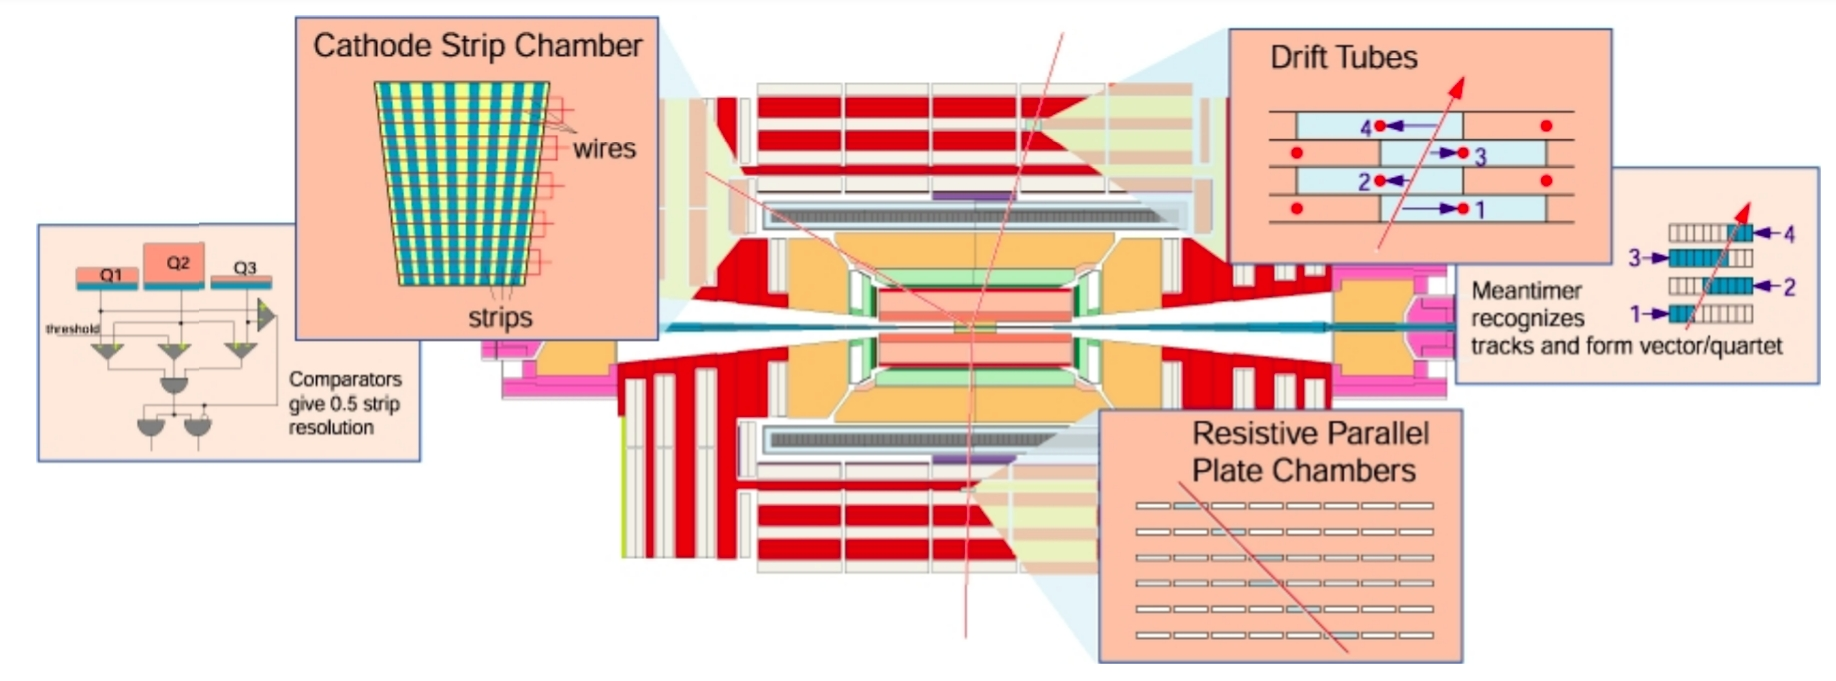
\includegraphics[scale=0.2]{images/ms}
\caption{The Muon System}
\label{fig:tms}
\end{figure}
The CSC and DT give accuracy in position checks while time measurements are identified using RPC.\\
\subsection{Pattern Recognition}
All particles except electron proton and neutron produced in CMS are generally unstable and they decay into lighter, more stable and well identified particles. Particles transversing along the tracker leave their characteristic signatures (patterns), after which they are uniquely identified in each layer they pass through. If any new particle is present or not can then be concluded, as shown in Fig.\ref{fig:patt}.\\
\subsection{Trigger System}
A trigger is a system which decides the events selection when specific number of events of the total can be recorded. Each detector has its own trigger system; Level-1 (L1) system is based on electronics and High Level Trigger (HLT) system is based on reconstruction software. For better probability of rare particle production, e.g. Higgs boson, bunch of protons are made to have $4 \times 10^{7}$ collisions per second. The different particles signatures resulting from these interactions are computed with high precision to save (or ‘trigger on’) events ($\sim 100/s$) which confirm Standard Model elementary particles and verify new physics, i.e. $\PHiggs \rightarrow ZZ^{*} \rightarrow 4l$. The event rate is therefore decreased to a tractable level. Subsequently, detailed analysis is performed on these separated events.\\
\begin{figure}[h]
\centering
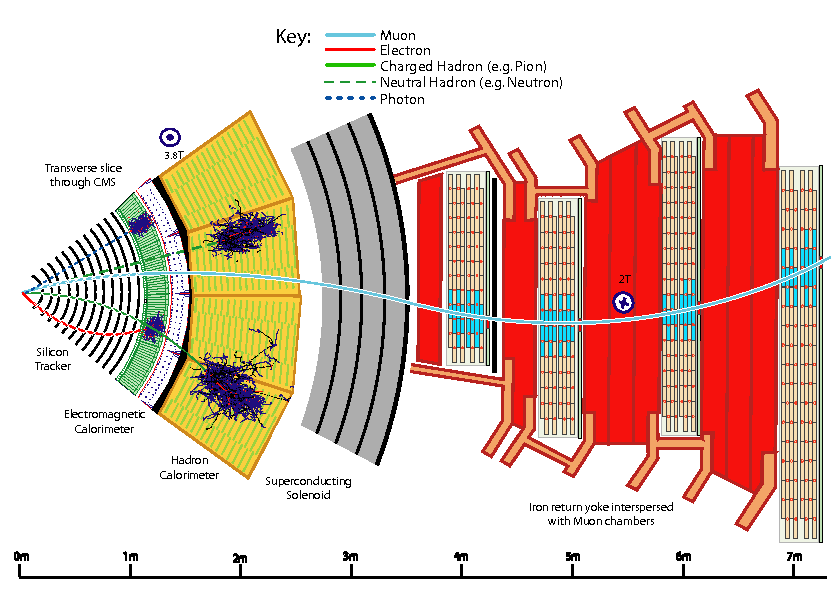
\includegraphics[scale=0.4]{images/pattern.png}
\caption{Pattern Recognition}
\label{fig:patt}
\end{figure}
\section{Co-ordinate System}
For object reconstruction in CMS experiment there is a standardized coordinate system. The centre point of the accelerator is the origin, x axis is directed towards the centre of the LHC ring, y axis points above and the z axis coincides with the beam direction, overall a 90$^{\circ}$ coordinate system. It is a cylindrical coordinate system; the x-y plane representing the transverse plane, azimuthal angle $\phi$ is measured between x axis and the x-y plane in the domain [$-\pi,\pi$] and lastly, the polar angle $\theta$ is calculated from the z axis in the domain [0, $\pi$].\\
The transverse plane displays the trajectories of particles in search for physics Beyond Standard Model (BSM). The y and x components of momentum and energy are measured at $90^{\circ}$ to the principal axis for for momentum and energy values (for massless particle $E_{T} = p_{T}$). The magnitude of projection vector of any transverse momentum $p_T$ component p onto transverse plane is given as:
\begin{equation}
    \label{eq1}
    P_{T} = \sqrt{P_{x}^{2}+P_{y}^{2}}
\end{equation}
The particle rapidity is calculated as:
\begin{equation}
    y = \frac{1}{2}ln\frac{(E+p_{z})}{(E-p_{z})}
\end{equation}
and when mass is neglected when compared to energy, m/E$\ll$1, it approaches the pseudo-rapidity:
\begin{equation}
    \eta = \frac{1}{2}ln\frac{(E+p_{z})}{(E-p_{z})} = -\frac{1}{2}tan\frac{\theta}{2}
    \end{equation}
which we will use in our thesis for electrons and muons. As the detector has cylindrical shape, the coordinate $\eta$ makes the contrast between two of the sub-detectors: 2 forward sections on opposite sides known as ``endcaps" and the central part ``barrel".\\
$\triangle R$ demonstrates the azimuthal angles $\phi_{i}$, which gives the angular distance between two particles, and pseudo-rapidity $\eta_{i}$, which is written as:
\begin{equation}
    \triangle R = \sqrt{(\eta_{1}-\eta_{2})^{2}+(\phi_{1}-\phi_{2})^{2}}
    \end{equation}
Total transverse energy calculation shows disparity, when a particle escapes the detection, this disparity is expressed as the transverse missing momentum $p^{miss}_{T}$. It is the total negative momentum of projection of reproduced objects on the x-y plane, and in the hermetic (sealed) detector, it is concluded to be the sum of neutrinos $p_T$. 